\documentclass{beamer}
\usetheme{Hannover}
\usepackage{amsmath}
\usepackage{amssymb}
\usepackage{amsthm}
\usepackage{graphicx}
\usepackage{pgf}
\usepackage{tikz}

% Definitions
\def\qqq{\mathbb{Q}}
\def\rrr{\mathbb{R}}
\def\zzz{\mathbb{Z}}
\def\fff{\mathbb{F}}
\def\gftwo{\mathbb{F}_2}
\def\zzzp{\mathbb{Z}_p}
\def\zzzn{\mathbb{Z}_N}
\def\zg{\mathbb{Z}_g}
\def\nnn{\mathbb{N}}
\def\BF{\mathcal{BF}}
\def\xn{(x_n)}
\def\yn{(y_n)}
\def\zn{(z_n)}
\def\an{(a_n)}
\def\Chi{\raisebox{2pt}{$\chi$}}
% \def\qed{$\Box}
% \newcounter{padic}

\begin{document}
\title{Analysis of Pseudorandom Sequences}
\author{Charles Celerier}
\frame{\titlepage}
\frame{\tableofcontents}

\section{Introduction}
\subsection{What is a pseudorandom sequence?}
\begin{frame}{What is a pseudorandom sequence?}
  \begin{itemize}
    \item uniform distribution
    \item low auto-correlation
  \end{itemize}
\end{frame}

\subsection{Stream Ciphers}
\begin{frame}{Stream Ciphers}
  \begin{tabular}{c c c c}
              & 01001110010000110101010101010010 & = & NCUR\\
              \pause
     $\oplus$ & 00000101000010010001100100000010 & \\
              \hline 
              \pause
              & 01001011010010100100110001010000 & = & KJLP
  \end{tabular}
\end{frame}

\begin{frame}{Why use stream ciphers?}
  \begin{itemize}
    \item fast
    \item easy to implement with hardware
    \item plaintext length is not always known
    \item near one-time-pad security
  \end{itemize}
\end{frame}

\begin{frame}{My research}
  \begin{itemize}
    \item Boolean functions
    \item 2-adic integers
    \item pseudorandom sequences
    \item shift registers
  \end{itemize}
\end{frame}

\section{Boolean Functions}
\subsection{GF(2)}
\begin{frame}{$\gftwo$ or ``GF two''}
  \begin{table}[h!]\label{tab:GF(2)}
    \centering
    \begin{tabular}{|c|c|}
      \hline
      XOR&AND\\
      \hline
      $0\oplus0:=0$&$0\cdot0:=0$\\
      $0\oplus1:=1$&$0\cdot1:=0$\\
      $1\oplus0:=1$&$1\cdot0:=0$\\
      $1\oplus1:=0$&$1\cdot1:=1$\\
      \hline
    \end{tabular}
  \caption{Binary Operations for $\gftwo$}
  \end{table}
\end{frame}

\begin{frame}{$\gftwo^n$ or ``GF two to the n''}
\begin{example}
  Let $a,b\in\gftwo^3$ such that $a=(1,0,1)$ and $b=(0,1,1)$ then
  \begin{align*}
    a+b      &=(1\oplus0,0\oplus1,1\oplus1)=(1,1,0) \\
  a\cdot b &=1\cdot0\oplus0\cdot1\oplus1\cdot1=1
  \end{align*}
\end{example}

\begin{fact}
  $\gftwo^n$ is a vector space.
\end{fact}
\end{frame}

\begin{frame}{Properties of $x\in\gftwo^n$}
  \begin{definition}
  \label{def:Hamming}
  	Let $x,y\in\gftwo^n$. Then $wt:\gftwo^n\rightarrow\nnn\cup\{0\}$
    is defined by
  	\[
  	  wt(x):=\sum_{i=0}^{n-1}x_i
  	\]
  	and $d:\gftwo^n\times\gftwo^n\rightarrow\nnn\cup\{0\}$ is defined by
  	\[
  	  d(x,y):=w(x+y).
  	\]
  	Then $wt(x)$ is the {\em Hamming\ weight} of $x$ and $d(x,y)$ is the
  	{\em Hamming\ distance} between $x$ and $y$.
  \end{definition}
\end{frame}
  
\begin{frame}{Some examples}
  \begin{example}
  	Let $a,b,c\in\gftwo^5$ such that
  	\[
  	a=(0,1,1,0,1),\ b=(1,1,1,0,0),\ {\rm and}\ c=(0,0,1,1,0).
  	\]
  	Then,
  	\begin{center}
  		\begin{tabular}{c c}
  			$wt(a)=3$&$d(a,b)=2$\\
  			$wt(b)=3$&$d(a,c)=3$\\
  			$wt(c)=2$&$d(b,c)=3$.\\
  		\end{tabular}
  	\end{center}
  \end{example}
\end{frame}

\subsection{Boolean Functions}
\begin{frame}{Boolean functions in $\BF^n$}
  \begin{definition}
  \label{def:boolean-function}
    Any function $f$ defined such that 
    \begin{equation*}
      f:\gftwo^n\rightarrow\gftwo
    \end{equation*}
    is a {\em Boolean function}. The set of all Boolean functions on $n$
    variables will be denoted by $\BF_n$.
  \end{definition}
\end{frame}

\begin{frame}{An example}
  \begin{example}
    Let $f=x_0+x_1$.
    \begin{table}
    \label{tab:truth-table}
    	\centering
      \begin{tabular}{|c|c||c|}
        \hline
        $x_0$&$x_1$&$f(x_0,x_1)$\\
        \hline
        0&0&0\\
        1&0&1\\
        0&1&1\\
        1&1&0\\
      	\hline
    	\end{tabular}
    	\caption{Truth Table of $f$}
    \end{table}
  \end{example}
\end{frame}

\subsection{Discrete Fourier Transforms}
\begin{frame}{Characters of $\gftwo^n$}
  \begin{definition}
    A {\em character} $\Chi$ of a finite abelian group $G$ is a group
    homomorphism from $G$ into a multiplicative group of complex numbers.
  \end{definition}
  \begin{fact}
    $\Chi_\lambda(x):=(-1)^{\lambda\cdot x}$ where $\lambda,x\in\gftwo^n$ is a
    {\em group\ character} of $\gftwo^n$.
  \end{fact}
\end{frame}

\begin{frame}{Discrete Fourier Transform}
  \begin{definition}\label{def:DFT}
    The {\em discrete\ Fourier\ transform} or DFT of a Boolean function is
    defined by
    \begin{equation}\label{eqn:DFT}
      \mathcal{F}f(\lambda)
        =\sum_{x\in\gftwo^n}f(x)\Chi_\lambda(x)
  	\end{equation}
  \end{definition}
\end{frame}

\begin{frame}{Pseudo Boolean Functions}
  \begin{definition}
    $\hat{f}(x):=(-1)^{f(x)}$ and $\hat{\BF}=\{\hat{f}:f\in\BF\}$.
  \end{definition}
  \begin{lemma}
    The characters of $\gftwo^n$ are functions in $\hat{\BF}_n
    =\{\hat{f}:f\in\BF_n\}$ and form an orthonormal basis of that set.
  \end{lemma}
\end{frame}

\begin{frame}
  \begin{lemma}
  \begin{equation}\label{eqn:rewrite-pseudo}
  	\hat{f}(x)
      =\frac{1}{2^{n/2}}
        \sum_{\lambda\in\gftwo^n}c(\lambda)\Chi_\lambda(x)
  \end{equation}
  	where $c(\lambda)$, the {\em Fourier\ coefficients} of $\hat{f}(x)$ are
    given by
    \begin{equation}\label{eqn:clambda}
      c(\lambda)=\frac{1}{2^{n/2}}\mathcal{F}\hat{f}(\lambda).
        %=\frac{1}{2^{n/2}}\sum_{x\in\gftwo^n}(-1)^{f(x)+\lambda\cdot x}.
    \end{equation}
  \end{lemma}
\end{frame}

\subsection{Bent Functions}
\begin{frame}{Rothaus' Definition and First Theorem}
  \begin{definition}\label{def:bent-function}
    If all of the Fourier coefficients of $\hat{f}$ are $\pm1$ then
    $f$ is a {\em bent\ function}.
  \end{definition}
  \begin{theorem}\label{thm:deg-of-bent-function}
  	If $f$ is a bent function on $\gftwo^n$, then $n$ is even, $n=2k$;
  	the degree of $f$ is at most $k$, except in the case $k=1$.
  \end{theorem}
\end{frame}

\begin{frame}{Properties of Bent Functions}
  \begin{enumerate}[1.]
    \item perfectly non-linear
    \item nearly balanced
    \item derivative is balanced
  \end{enumerate}
\end{frame}

\section{2-adic integers}
\begin{frame}{Question}
  What happens when we write positive integers with infinitely many digits? \\
  \pause
  You get elements of $N$-adic integer rings!
\end{frame}

\begin{frame}{$\zzz_2$}
  \begin{align*}
    1&=1000\cdots\\
    2&=0100\cdots\\
    3&=1100\cdots\\
    -1&=1111\cdots\\
    1/3&=1101010101\cdots\\
    -1/3&=1010101010\cdots
  \end{align*}
  \par I am intentionally skipping the details of how to construct rational
  numbers such as $1/3$. It is only important to know that as long as the
  denominator is not divisble by 2, it can be done.
\end{frame}

\begin{frame}
  \begin{definition}
    Let $\alpha=\an\in\zzz_2\setminus(0)$. If $m$ is the smallest number in
    $\nnn\cup\{0\}$ such that $a_m \not\equiv 0 \pmod 2^{m+1}$, then the {\em
    2-adic\ valuation} of $\alpha$ is $m$, or $\log_2(\alpha)=m$. If $\alpha=0$,
    thenssss$\log_2(\alpha)=\infty$.
  \end{definition}
  \begin{example}
    Let $\alpha=0001011101111\cdots$. Then $\log_2(\alpha)=3$.
  \end{example}
\end{frame}

\section{Boolean Sequences}
\begin{frame}{Boolean Sequences}
  \begin{definition}
    Let $(a_n)$ be a sequence. If $T$ is the smallest integer such that
    $a_i=a_{i+T}$, then the {\em minimal\ period} of $(a_n)$ is $T$.
  \end{definition}
  
  \begin{definition}\label{def:lex-Bool-seq}
    Let $f\in\BF_n$ and $v_i\in\gftwo^n$ such that $v_i=B^{-1}(i)$ for
    $0\leq i<2^n$. Then,
    \begin{equation}
      seq(f)=(f(v_0),f(v_1),\cdots,f(v_{2^n-1}),f(v_0),\cdots)
    \end{equation}
    is a {\em lexicographical\ Boolean\ sequence}.
  \end{definition}
\end{frame}

\begin{frame}{2-adic Expansion}
  \begin{definition}\label{2-adic-ex}
    Let $f\in\BF_n$ and $v_i\in\gftwo^n$ such that $v_i=B^{-1}(i)$ for
    $0\leq i<2^n$. Then,
    \begin{equation}
      \alpha_f=(f(v_0),f(v_0)+f(v_1)\cdot2,\cdots,\allowbreak
        f(v_0)+\cdots\allowbreak+f(v_i)\cdot2^i,\allowbreak\cdots)
    \end{equation}
    where $\alpha_f\in\zzz_2$ is called the {\em 2-adic\ expansion} of $f$.
  \end{definition}
  
  \begin{lemma}
    The digit representation of $\alpha_f$ is $seq(f)$.
  \end{lemma}
\end{frame}

\section{Shift Registers}
\begin{frame}{LFSR}
  \begin{figure}[h!]
    \centering
    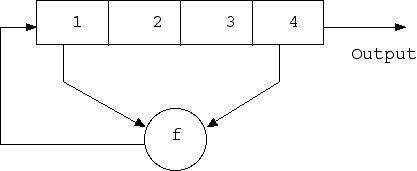
\includegraphics[totalheight=0.5\textheight]{lfsr.jpg}
    \caption{Linear Feedback Shift Register from Google Images}
  \end{figure}
\end{frame}

\begin{frame}{Eventually periodic shift registers}
  \par Solomon W. Golomb wrote the famous book \textit{Shift Register
  Sequences} in 1967 which contain numerous elementary facts about finite
  state machines.
  \begin{theorem}\label{thm:golomb-2}
    If the input sequence to a finite state machine is eventually periodic, then
    the output sequence is eventually periodic.
  \end{theorem}
\end{frame}

\subsection{Breaking a Stream Cipher}
\begin{frame}{Breaking a Stream Cipher}
  \par \textit{Kerckhoffs' principle}: ``In assessing the security of a
  cryptosystem, one should always assume the enemy knows the method being
  used.''
  \par Typically, breaking a stream cipher will mean recovering the state of
  the shift register at a given time.
\end{frame}

\begin{frame}{State of the register}
  \begin{figure}[h!]
    \centering
    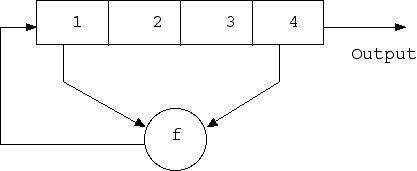
\includegraphics[totalheight=0.5\textheight]{lfsr.jpg}
    \caption{Linear Feedback Shift Register from Google Images}
  \end{figure}
\end{frame}

\section{Pseudorandom Sequences of 0s and 1s}
\subsection{Analyzing}
\begin{frame}{Two Methods}
  \begin{enumerate}[1.]
    \item 2-adic integers
    \item Boolean sequences
  \end{enumerate}
\end{frame}

\subsection{Constructing}
\begin{frame}{Maiorana-McFarland Class Boolean Functions}
  \par A simple bent function construction is accomplished by the Boolean
  functions in the {\em Maiorana-McFarland\ class}. This is the the set
  $\mathcal{M}$ which contains all Boolean functions on
  $\gftwo^n=\{(x,y):x,y\in\gftwo^{n/2}\}$, of the form:
    \[
    f(x,y)=x\cdot\pi(y)\oplus g(y)
    \]
  where $\pi$ is any permutation on $\gftwo^{n/2}$ and $g$ any Boolean
  function on $\gftwo^{n/2}$.\\
  
  \par All functions in the Maiorana-McFarland class of Boolean functions are
  bent.
\end{frame}
  
\begin{frame}{Using Bent functions for Boolean Sequences}
  \begin{theorem}
    The lexicographical Boolean sequence of a Bent function has a period
    exactly $2^n$.
  \end{theorem}
\end{frame}

\begin{frame}
  \par Consider the subset of Maiorana-McFarland class Boolean functions where
  $g(y)=0$. $\bar{\pi}$ will be the function which specifies where each
  index moves to under the permutation $\pi$.
  
  \begin{theorem}
    $\log_2(\alpha_{x\cdot\pi(y)})=2^{n/2}+2^{\bar{\pi}(y_0)}$
  \end{theorem}

  \par The 2-adic valuation of the Boolean sequence of the functions in this
  subset is entirely dependent on the permutation $\pi$.
\end{frame}

\section{Conclusion}
\begin{frame}{Conclusion}
  \begin{itemize}
    \item Pseudorandom sequences
    \item Stream Ciphers
    \item Analysis using Boolean functions and 2-adic integers
    \item Connections between Bent functiosn and 2-adic valuation
  \end{itemize}
\end{frame}

\begin{frame}{Questions?}
  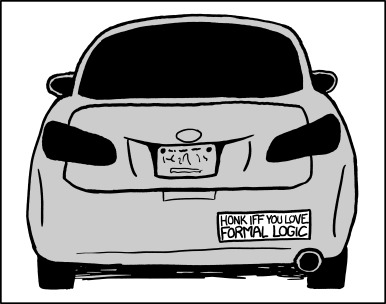
\includegraphics[totalheight=.98\textheight]{formal_logic.jpg}
\end{frame}

\end{document}
